

%% Based on the style files for ACL-2013, which were, in turn,
%% Based on the style files for ACL-2012, which were, in turn,
%% based on the style files for ACL-2011, which were, in turn, 
%% based on the style files for ACL-2010, which were, in turn, 
%% based on the style files for ACL-IJCNLP-2009, which were, in turn,
%% based on the style files for EACL-2009 and IJCNLP-2008...

%% Based on the style files for EACL 2006 by 
%%e.agirre@ehu.es or Sergi.Balari@uab.es
%% and that of ACL 08 by Joakim Nivre and Noah Smith

\documentclass[11pt]{article}
\usepackage{acl2014}
\usepackage{times}
\usepackage{url}
\usepackage{latexsym}

% graphs
\usepackage{graphicx, wrapfig}
\usepackage{subcaption}
\usepackage{float}
\usepackage{tabularx}

% FANCY GRAPHS WITH LATEX
\usepackage{pgfplots}
\pgfplotsset{compat=1.16}
\usepackage{tikz}

%Tables
\usepackage{booktabs}



%\setlength\titlebox{5cm}

% You can expand the titlebox if you need extra space
% to show all the authors. Please do not make the titlebox
% smaller than 5cm (the original size); we will check this
% in the camera-ready version and ask you to change it back.


%%%%%%%%%%%%%%%%%%%%%%%%%%%%%%%%%%%%%%%%%%%%%%%%%%%%%%%%%%%%%%%%%%%%%%%%%%%%%%%%%%%%%%%%%%%


\title{Gender Bias in Fairy Tales}

% I think we just add the uva mail addresses here, seems the best for this paper no? 
\author{
    Lisa van Gelderen \\
  {\tt lisa.van.gelderen@student.uva.nl} \\
    Alexia Muresan \\
  {\tt alexia.muresan@student.uva.nl} \\
    Zoë Prins \\
  {\tt zoë.print@student.uva.nl} \\
    Victor van der Sman \\
  {\tt victor.van.der.sman@student.uva.nl} \\}

\date{}

\begin{document}
\maketitle
\begin{abstract}
% Victor
  Fairy tales can give children important lessons about life and the world that they live in and are mostly viewed as such. In the western world one is unlikely to find a single person that does not know the story of Snow White and many of the other famous fairy tales. These stories however often contain messages about gender roles, even though these messages might be based on outdated stereotypes \cite{Lieberman}. A lot of children grow up hearing fairy tales before bed, or they learn reading by virtue of fairy tales. As such, these stories can have a big impact on the forming of opinions in young children \cite{Wardetzky}. We map and visualize the gender bias found in fairy tales by analyzing a corpus of European fairy tales written largely by the brothers Grimm \cite{Aho:10}. Using bi-grams, n-grams, a ppmi space and a Gensim Word2Vec model to show that gender bias exists on multiple levels in most fairy tales. Not only are women represented mostly as passive agents that require male characters to drive them forward, we show that female characters are largely characterized by their outward appearance instead of personality. 
\end{abstract}


\section{Introduction}

% Victor
Many of the fairy tales found today can be traced back to the bundles released by the brothers Grimm more than a hundred years ago. These stories were originally an oral tradition by female spinners in predominantly German lands. These oral stories often contained themes of rape or male oppression, and were a way for the women to stay awake while spinning. But after the brothers Grimm kept changing the stories to appeal to a larger audience, these themes were largely replaced and removed until the stories more reflected the views of 19th century patriarchal men \cite{Marshall}

Studies about the views of children suggest their views on gender can be heavily influenced by reading certain fairy tales \cite{Wardetzky}. It is therefore worth to investigate the way these stories handle gender roles. In old stories, gender roles can be quite stereotypical and patronizing towards women. The most classic fairy tale template is a great example of this: “A brave prince needs to rescue a beautiful but helpless princess from her perils.”. Gender bias in fairy tales include more focus on beauty in female characters and less on intelligence, portraying female characters as passive agents. If we teach children values with stories that contain stereotypical gender roles, these roles will be perpetuated in the next generation. This is why we aim to map the way fairy tales deal with gender in order to better understand and shed light on the problem. 
 
\section{Related Work}

% Alexia
There has been significant research about the stereotypical portrayal of female characters in fairy tales, enforcing traditional gender roles. Across this genre women are  clearly represented as the inferior gender, ingraining these biases in the minds of children who are to become yet another generation that accepts and cultivates gender bias. Central to these stories is the appearance of female characters, considered “a girl's most valuable asset, perhaps her only valuable asset” (Lieberman, 1972). Their "beauty is their wealth” \cite{Weingart}, observable through lengthy descriptions of female characters’ appearance, building towards a shallow representation of women. Interestingly, throughout fairy tales appears the “stereotype that a woman’s character is directly tied to her appearance" (Neikirk, 2013). Beauty appears to ultimately determine the value of a woman; “Girls win the prize if they are the fairest of them all; boys win if they are bold, active, and lucky” (Lieberman, 1972). This pattern repeats itself in many  stories, opposing Snow White and the 'hideous' witch, Cinderella and her ugly step-sisters... Secondly, female characters’ life revolves around the man in the story. Lieberman says that most of these “stories focus upon courtship, which is magnified into the most important and exciting part of a girl's life [and] marriage is the fulcrum and major event of nearly every fairy tale”. It is always the happy ending, as if marriage is all a woman could ever want and need in order to be happy and fulfilled. “The passive heroine has no ambitions beyond marriage and through the lens of romance, ideas about gender roles are formed” (Meland, 2020). Most problematic is that women are depicted as a passive gender: “heroines are chosen for their beauty [...], not for anything they do [...], they seem to exist passively until they are seen by the hero” (Lieberman, 1972). This global image of women in fairy tales puta forward “traits that are supposedly inherently feminine: beauty, goodness, passivity, dependence, and an affinity for the domestic sphere” \cite{Weingart}. There are few examples (if any) of strong, determined and capable female characters in fairy tales; “What is praiseworthy in males, however, is rejected in females [and] being powerful is mainly associated with being unwomanly” (Lieberman, 1972). This cultivates gender bias (criticism of “the active, ambitious, "pushy" woman” (Lieberman, 1972) that is still present nowadays) and leaves young girls without role models. Some go as far as to say that they "perpetuate Christian, patriarchal concepts as a means of maintaining the gender hierarchy” (Neikirk, 2013). Overall, fairy tales cultivate traditional gender roles, visible in the reactions of schoolchildren and teachers to an adapted production of the Princess and the Pea. Gender roles were switched, creating a princess characterised by her “physical strength and activity, her loudness, and facial expressions and lack of silence” (Meland, 2020), deemed confusing by the audience. Conversely, “the king was wearing pink and red, it was weird!’ (Meland, 2020), claimed one of the teachers. This shows just how much traditional fairy tales influence what is perceived as ‘normal’ for both genders, “suggesting to [children] the limitations that are imposed by sex upon a person's chances of success in various endeavors” (Lieberman, 1972). 



\section{Data set}

% Alexia
The dataset used here is a fairy tale corpus from INESC-ID's Human Language Technology Lab. It is sematically organised and PoS-tagged, and contains fairy tales by five different authors, organized in clusters. The database also provides the following information:

\begin{table}[H]
\centering
\begin{tabular}{@{}ll@{}}
\toprule
Number of stories           &   453         \\ \midrule
Number of words             &   908,174     \\
Average words/story         &   1891        \\
Words/shortest story        &   75          \\
Words/longest story         &   17,694      \\
Clusters                    &   365         \\ \bottomrule
\end{tabular}
\label{ml_features}
\end{table}
 
In addition to the above-mentioned dataset, another dataset that we assembled ourselves with stories has also been used. This can be found in the andersongrimm.txt file. The stories in that file come from project Gutenberg.

\section{Method}

% Lisa 
In order to work with the data, some additional preprocessing was performed. This consisted of putting all stories from the dataset in one list, removing non-lemmatized words, stopwords, white space and unnecessary tokens such as punctuation. Numeric characters and irrelevant word categories (conjunctions, determinants and prepositions) were filtered out, and the remaining tokens were converted to lowercase.\par
With the data now processed as needed, a small analysis using an n-gram model was used to generate small pieces of text based on the dataset. This was done to see if the generated text would have clear biases, which would indicate that the test the model was trained on has biases (or not) as well. Additionally, an inspection of frequent bigrams was performed to see if specific words were more commonly paired with a specific gender.  \par
Secondly, an analysis using word embeddings was performed. This method focused on analysing surface co-occcurence by counting how many times a contextual word occurs in a collocational span surrounding the target word, in a symmetric 5 word span. After which, a similarity matrix was created based on the cosine similarity. \par
Finally, a Word2Vec model was trained based on the dataset to look again at the similarities between two words. Based on this model, a scatterplot was created to see how close two words are. 

\subsection{models}

The first model used was an n-gram model trained on the Anderson and Grimm fairy tales. The models was designed to generate text of a specified length. In order to do this, the model took n-grams as input (by testing it was found that 8-grams produced the best results), and created a dictionary with the n-grams and a counter. Based on this counter, a probability was assigned to each word that that word followed another. When asked to generate text, the model choose randomly from a list of options or words to follow the previous, but gave the more likely words a higher chance of being chosen. \par
The second model was the Word2Vec model with parameters as specified in the Word2Vec\_FastText\_Comparison, and preprocessed sentences as input. For the full code, see the github repository with a single code file containing a partial narrative of all coding of the entire research: \url{https://github.com/lisavangelderen/FairyTale} 

\section{Results}
% Victor

As to not subject the paper to endless tables most of the results are kept in the notebook of the repository. We explain the interesting parts of our results here. In the notebook there are a number of figures that were also omitted from the paper. 

In our \textbf{bi-gram analysis} we found women to be more likely to be described as beautiful than men, but less likely to be called strong or fighting. We also found the fact that women are twice as likely to be described as old, something Weingart and Jorgensen go into more depth about. Interesting about this is that while both men and women get called old as the most used adjective, women are more often described as old than they say anything. Which is telling about the descriptive role women take in fairy tales. Rather than speak or act, these women are described. This is highlighted even more in the "king" "queen" relationship. According to the co-occurrences (\ref{king/queen} a queen can be seen as occurring mainly either next to a king or in her role as mother, with the most occurring adjective for a queen being "little" and "young". Whereas the king is "great" and has mainly active verbs in his occurrences.

\begin{table}[H]
\centering
\begin{tabular}{@{}lll@{}}
\toprule
                    &           king        \\ \midrule
say                 &           7044        \\
son                 &           5108        \\
daughter            &           4938        \\ 
king                &           3382        \\
come                &           2484        \\
go                  &           2344        \\
would               &           1658        \\
great               &           1580        \\
take                &           1557        \\            
go                  &           1503        \\ \bottomrule
           
\end{tabular}
\hspace*{0.5cm}
\begin{tabular}{@{}lll@{}}
\toprule

                    &       queen   \\ \midrule
king                &       1227    \\
say                 &       803     \\
gulnare             &       632     \\ 
go                  &       479     \\
child               &       410     \\
young               &       397     \\
mother              &       397     \\
one                 &       376     \\
little              &       339     \\            
queen               &       338     \\ \bottomrule
\end{tabular}

\caption{Comparing king and queen co-occurrences}
\label{king/queen}
\end{table}

In addition to bi-grams we also made use of an \textbf{n-gram model} to create short stories. Even though most of the stories were quite incoherent and could not see further than a single sentence, at some points these stories exposed bias quite clearly. One of the stories starts of with {\em"At home the beautiful wife prayed for her husband and her father"}, Showing how the woman cannot act but instead must hope for the return of her family (but at least she's beautiful). That same story ends when the neighbours enters through the door, again it is the male that takes action to drive the plot, and exclaims something. The final sentence being: {\em"To travel! to travel!. exclaimed he,  overcome by most painful and passionate remembrances. But he did not despair. This was capital."}. 


We also noted something interesting when looking at the \textbf{ppmi space} for the different genders. While this metric corrects for high frequency words, it showed that "woman" is mostly occurring next to "man" or "king". The same can be seen for "girl" or "queen", all of these words have a very high likelihood to be written next to their male counterparts. While this on it's own is not unusual, men and women can be used quite often together in text. The bias however comes in when reversing this analysis. For "men", "woman" is only the 7th most occurring word, for "king", "woman" is not even in the 20 most likely in the ppmi space. This trend continues with different male and female words such as "boy/girl", "prince/princess" or even just "male/female".

\begin{figure}{L}
    \centering
    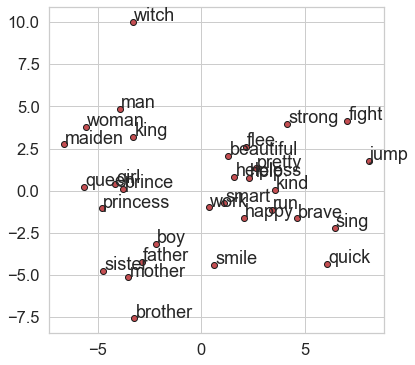
\includegraphics[scale=0.40]{PCA_ScatterPlot.png}
    \caption{\label{fig:PCA} PCA Scatterplot created by the gensim model depicting a 2-dimensional representation of the word embeddings.}
\end{figure}

For the \textbf{Gensim model} we noted more of the same results, but to a much lesser extent than on the other metrics. With the similarities created by the model we can also see that girls are more similar to woodcutters than boys are, something we did not entirely expect as it is traditionally a job for men involving a lot of physical strength. This can also be caused by the removal of stopwords, causing these two words to be close together in the filtered data, but not in the original sentence. \par
Based on the wordvectors, figure \ref{fig:PCA} was obtained after a PCA. 

\section{Conclusion}
%Victor

In our paper we aim to answer the question of whether or not gender bias exists in fairy tales. This is a question with a binary response, and our response to this question is a resounding "yes". Not the least of which due to the fact that this question has been answered numerous times by other qualified researchers \cite{Baker} \cite{Lieberman} \cite{Weingart}. This does not devalue or paper however, as there is value in the repetition of scientific research. We hope to add something to the theory by building on this research and confirming it. In our results we found varying degrees of the same results as these previous papers. 

From the bi-gram analysis we showed the dependency a queen has on her king while the king goes where he pleases. One can imagine that many young women will look up to the position of queen, as it is quite well known to be the highest female "rank" in the story. From this implicit message these children will understand that to achieve the highest "rank" in life they will have to behave accordingly and thus stay passive. For young boys this message is quite different and has a completely different effect. 

In the 2 sentences shown from the n-gram analysis the story shows all that is we find troubling with the gender bias of these models. Having learned from the fairy tales that female characters wait and look "beautiful", whereas male characters act, travel and overcome. From this we can conclude a quite clear theme in the stories where female character development is almost entirely driven by interaction with their male counterparts. While the male characters have a lot more freedom to develop and take action on their own. This is also supported by the ppmi analyses showing female words being much more inclined to be with males than vice versa. 

These points add to the mounting pile of research collaborating to the fact that there is definitely certain gender bias in these stories. We found however that the results were not as obvious as previously expected, our Gensim Word2Vec model on some occasions even went completely against the grain of traditional stereotypes. 

% \subsection{Discussion}


\section{Future Work}

% Victor
Here we can give ideas on how our work can be expended on by researchers in the future that can use the information we found to do the things we did not have the resources or time to look into. There were multiple things that we found while working that, given time, we wanted to look into and explore more. 

One of these things is the male gender bias in these stories. In our paper we mostly look at female oppression and stereotypes, we were not the first to do this and will likely not be the last. But the stories we looked into were mostly written/adapted in a society that wasn't entirely good for men either. Even though the men are represented and portrayed a lot more favourable in the stories than women are. The male characters are taught to be brave, this implicitly sends the message that fear is then inherently something to avoid. This, combined with more, similar, themes, add to the toxic masculinity culture present in our society today. 

Another interesting idea to expand on in the future can be the creation of stories similar to how previous work has done with children \cite{Wardetzky}. While we created short sentences using an n-gram model, this could be expanded on. Making a model, trained on fairy tales, write short fairy tale when given a certain amount of words could expose the same bias found in children. 

For all results and code (not) displayed in the paper see\footnote{https://github.com/lisavangelderen/FairyTale}.





\begin{thebibliography}{}

% Victor
\bibitem[\protect\citename{Aho and Ullman}1972]{Aho:10}
Vaz Lobo, Paula  and  de Matos, David~M.
\newblock 2010.
\newblock {\em Fairy Tale Corpus Organization Using Latent Semantic Mapping and an Item-to-item Top-n Recommendation Algorithm}.
\newblock European Language Resources Association (ELRA), Malta.


\bibitem[\protect\citename{Weingart and Jorgensen}2013]{Weingart}
Weingart, Scott and Jorgensen, Jeana
\newblock 2013.
\newblock {\em Computational Analysis of the Body in European Fairy Tales}.
\newblock Literary and Linguistic Computing/ (2013): 404-416.


\bibitem[\protect\citename{Meland}2020]{Torill}
Aud~T, Meland
\newblock 2020
\newblock {\em Challenging gender stereotypes through a transformation of a fairy tale Challenging gender stereotypes through a transformation of a fairy tale.}.
\newblock European Early Childhood Education Research Journal. 28.


\bibitem[\protect\citename{Marshall}2004]{Marshall}
Marshall~E. 
\newblock 2004d.
\newblock {\em The Daughter’s Disenchantment: Incest as Pedagogy in Fairy Tales and Kathryn Harrison’s “The Kiss.”}.
\newblock College English, 66(4), 403–426.

\bibitem[\protect\citename{Lieberman}1972]{Lieberman}
M.R. Lieberman
\newblock 1972.
\newblock {\em ""Some Day My Prince Will Come": Female Acculturation through the Fairy Tale."}.
\newblock College English. vol. 34, no.3, p.383


\bibitem[\protect\citename{Wardetzky}1990]{Wardetzky}
Wardetzky, K.
\newblock 1990.
\newblock {\em  The Structure and Interpretation of Fairy Tales Composed by Children. The Journal of American Folklore}.
\newblock The Journal of American Folklore, 103(408), 157–176.


\bibitem[\protect\citename{Baker-Sperry}2003]{Baker}
Baker-Sperry, Lori and Liz Grauerholz
\newblock 2003.
\newblock {\em The Pervasiveness and Persistence of the Feminine Beauty Ideal in Children's Fairy Tales}.
\newblock Gender and Society, pp. 711-726


\bibitem[\protect\citename{Neikirk}2013]{Neikirk}
Neikirk, A. 
\newblock 2013.
\newblock {\em ""...Happily Ever After" (or What Fairy Tales Teach Girls About Being Women"}.
\newblock Anthropology, 38-42.



\end{thebibliography}



\end{document}